\documentclass[12pt]{article}
\usepackage{tikz}
\usepackage{amsmath}
% Underlining package
\usepackage{ulem}
\usetikzlibrary{calc}
\usetikzlibrary{angles,quotes}
\usepackage[a4paper, portrait, margin=1cm]{geometry}
\usepackage{fancyhdr}

\newcommand{\HeadingQuestions}{%
\section*{\Large Name: \underline{\hspace{8cm}} \hfill Date: \underline{\hspace{3cm}}}%
\vspace{-3mm}\par
\textbf{Area Rectangles}\vspace{1pt}\hrule
}

% raise footer with page number; no header
\fancypagestyle{myfancypagestyle}{
  \fancyhf{}% clear all header and footer fields
  \renewcommand{\headrulewidth}{0pt} % no rule under header
  \fancyfoot[C] {\thepage} \setlength{\footskip}{14.5pt} % raise page number allowed min 14.5pt
}
\pagestyle{myfancypagestyle}  % apply myfancypagestyle

\newcounter{minipagecount}

\begin{document}
\HeadingQuestions
\vspace{8mm}

\begin{minipage}{0.55\textwidth}
  \refstepcounter{minipagecount}
  \noindent{(\theminipagecount)}\quad
 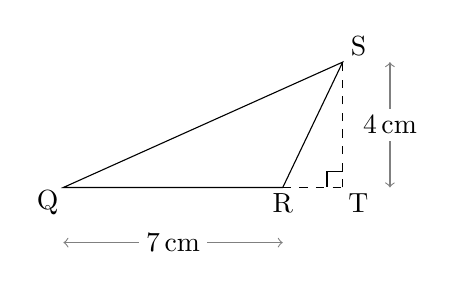
\begin{tikzpicture}[scale=1.0, baseline=(current bounding box.north)]
        \begin{scope}[rotate=0]

        \coordinate (Q) at (0,0);
        \coordinate (R) at (2.786,0);
        \coordinate (T) at ($(R)+(0.761,0)$);  % extend out
        \coordinate (S) at ($(T)+(0,1.592)$); % Perpendicular upwards

        \draw (Q)--(R)--(S)--cycle;
        \draw[dashed] (R)--(T);
        \draw[dashed] (T)--(S);
        \pic [draw, -, angle radius=0.2cm] {right angle=S--T--R};

        % Vertex LABELS
        % Labels relative to shape geometry
        \node at ($(Q)+(-0.2,-0.2)$) {Q};
        \node at ($(R)+(0.0,-0.2)$) {R};
        \node at ($(T)+(0.2,-0.2)$) {T};
        \node at ($(S)+(0.2,0.2)$) {S};


        % dotted/dashed arrows shifted away from edges
        % Horizontal side (A-B), shifted down yshift=0mm,
        \draw[<->, gray]
            ($(Q) + (0,-0.7cm)$) -- ($(R) + (0,-0.7cm)$)
            node[black, midway, fill=white, inner sep=2.5pt] {7\,cm};

        % Vertical side (D-C), shifted right xshift=0mm,
        \draw[<->, gray]
            ($(T)+(0.6,0)$) -- ($(T |- S)+(0.6,0)$)
            node[black, midway, fill=white, inner sep=2.5pt] {4\,cm};
    \end{scope}
\end{tikzpicture}
\end{minipage}%
\hfill
\begin{minipage}{.4\textwidth}
  \begin{align*}
    \text{Area} &= \frac{1}{2} \text{bh} \\
    \text{Area} &= \frac{1}{2} \times 7 \text{cm} \times 4 \text{cm}  \\
    \text{Area} &= \dotuline{~~~~~~~} \text{cm}^2
  \end{align*}
\end{minipage}

\par\vspace{1cm}\begin{minipage}{0.55\textwidth}
  \refstepcounter{minipagecount}
  \noindent{(\theminipagecount)}\quad
 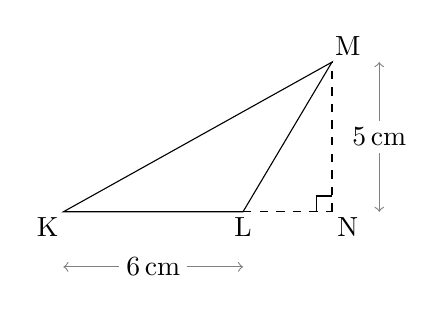
\begin{tikzpicture}[scale=1.0, baseline=(current bounding box.north)]
        \begin{scope}[rotate=0]

        \coordinate (K) at (0,0);
        \coordinate (L) at (2.281,0);
        \coordinate (N) at ($(L)+(1.13,0)$);  % extend out
        \coordinate (M) at ($(N)+(0,1.901)$); % Perpendicular upwards

        \draw (K)--(L)--(M)--cycle;
        \draw[dashed] (L)--(N);
        \draw[dashed] (N)--(M);
        \pic [draw, -, angle radius=0.2cm] {right angle=M--N--L};

        % Vertex LABELS
        % Labels relative to shape geometry
        \node at ($(K)+(-0.2,-0.2)$) {K};
        \node at ($(L)+(0.0,-0.2)$) {L};
        \node at ($(N)+(0.2,-0.2)$) {N};
        \node at ($(M)+(0.2,0.2)$) {M};


        % dotted/dashed arrows shifted away from edges
        % Horizontal side (A-B), shifted down yshift=0mm,
        \draw[<->, gray]
            ($(K) + (0,-0.7cm)$) -- ($(L) + (0,-0.7cm)$)
            node[black, midway, fill=white, inner sep=2.5pt] {6\,cm};

        % Vertical side (D-C), shifted right xshift=0mm,
        \draw[<->, gray]
            ($(N)+(0.6,0)$) -- ($(N |- M)+(0.6,0)$)
            node[black, midway, fill=white, inner sep=2.5pt] {5\,cm};
    \end{scope}
\end{tikzpicture}
\end{minipage}%
\hfill
\begin{minipage}{.4\textwidth}
  \begin{align*}
    \text{Area} &= \frac{1}{2} \text{bh} \\
    \text{Area} &= \frac{1}{2} \times 6 \text{cm} \times 5 \text{cm}  \\
    \text{Area} &= \dotuline{~~~~~~~} \text{cm}^2
  \end{align*}
\end{minipage}

\par\vspace{1cm}\begin{minipage}{0.55\textwidth}
  \refstepcounter{minipagecount}
  \noindent{(\theminipagecount)}\quad
 \begin{tikzpicture}[scale=1.0, baseline=(current bounding box.north)]
        \begin{scope}[rotate=90]

        \coordinate (E) at (0,0);
        \coordinate (F) at (5.717,0);
        \coordinate (H) at ($(F)+(1.283,0)$);  % extend out
        \coordinate (G) at ($(H)+(0,2.144)$); % Perpendicular upwards

        \draw (E)--(F)--(G)--cycle;
        \draw[dashed] (F)--(H);
        \draw[dashed] (H)--(G);
        \pic [draw, -, angle radius=0.2cm] {right angle=G--H--F};

        % Vertex LABELS
        % Labels relative to shape geometry
        \node at ($(E)+(-0.2,-0.2)$) {E};
        \node at ($(F)+(0.0,-0.2)$) {F};
        \node at ($(H)+(0.2,-0.2)$) {H};
        \node at ($(G)+(0.2,0.2)$) {G};


        % dotted/dashed arrows shifted away from edges
        % Horizontal side (A-B), shifted down yshift=0mm,
        \draw[<->, gray]
            ($(E) + (0,-0.7cm)$) -- ($(F) + (0,-0.7cm)$)
            node[black, midway, fill=white, inner sep=2.5pt] {8\,cm};

        % Vertical side (D-C), shifted right xshift=0mm,
        \draw[<->, gray]
            ($(H)+(0.6,0)$) -- ($(H |- G)+(0.6,0)$)
            node[black, midway, fill=white, inner sep=2.5pt] {3\,cm};
    \end{scope}
\end{tikzpicture}
\end{minipage}%
\hfill
\begin{minipage}{.4\textwidth}
  \begin{align*}
    \text{Area} &= \frac{1}{2} \text{bh} \\
    \text{Area} &= \frac{1}{2} \times 8 \text{cm} \times 3 \text{cm}  \\
    \text{Area} &= \dotuline{~~~~~~~} \text{cm}^2
  \end{align*}
\end{minipage}

\par\vspace{1cm}\begin{minipage}{0.55\textwidth}
  \refstepcounter{minipagecount}
  \noindent{(\theminipagecount)}\quad
 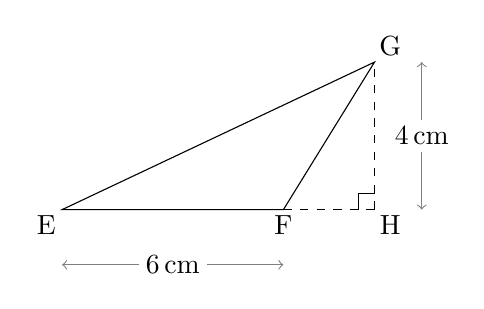
\begin{tikzpicture}[scale=1.0, baseline=(current bounding box.north)]
        \begin{scope}[rotate=0]

        \coordinate (E) at (0,0);
        \coordinate (F) at (2.811,0);
        \coordinate (H) at ($(F)+(1.157,0)$);  % extend out
        \coordinate (G) at ($(H)+(0,1.874)$); % Perpendicular upwards

        \draw (E)--(F)--(G)--cycle;
        \draw[dashed] (F)--(H);
        \draw[dashed] (H)--(G);
        \pic [draw, -, angle radius=0.2cm] {right angle=G--H--F};

        % Vertex LABELS
        % Labels relative to shape geometry
        \node at ($(E)+(-0.2,-0.2)$) {E};
        \node at ($(F)+(0.0,-0.2)$) {F};
        \node at ($(H)+(0.2,-0.2)$) {H};
        \node at ($(G)+(0.2,0.2)$) {G};


        % dotted/dashed arrows shifted away from edges
        % Horizontal side (A-B), shifted down yshift=0mm,
        \draw[<->, gray]
            ($(E) + (0,-0.7cm)$) -- ($(F) + (0,-0.7cm)$)
            node[black, midway, fill=white, inner sep=2.5pt] {6\,cm};

        % Vertical side (D-C), shifted right xshift=0mm,
        \draw[<->, gray]
            ($(H)+(0.6,0)$) -- ($(H |- G)+(0.6,0)$)
            node[black, midway, fill=white, inner sep=2.5pt] {4\,cm};
    \end{scope}
\end{tikzpicture}
\end{minipage}%
\hfill
\begin{minipage}{.4\textwidth}
  \begin{align*}
    \text{Area} &= \frac{1}{2} \text{bh} \\
    \text{Area} &= \frac{1}{2} \times 6 \text{cm} \times 4 \text{cm}  \\
    \text{Area} &= \dotuline{~~~~~~~} \text{cm}^2
  \end{align*}
\end{minipage}

\par\vspace{1cm}\begin{minipage}{0.55\textwidth}
  \refstepcounter{minipagecount}
  \noindent{(\theminipagecount)}\quad
 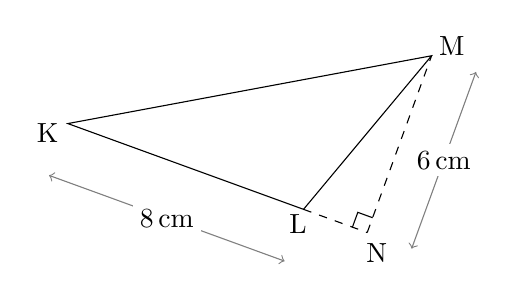
\begin{tikzpicture}[scale=1.0, baseline=(current bounding box.north)]
        \begin{scope}[rotate=-20]

        \coordinate (K) at (0,0);
        \coordinate (L) at (3.185,0);
        \coordinate (N) at ($(L)+(0.861,0)$);  % extend out
        \coordinate (M) at ($(N)+(0,2.389)$); % Perpendicular upwards

        \draw (K)--(L)--(M)--cycle;
        \draw[dashed] (L)--(N);
        \draw[dashed] (N)--(M);
        \pic [draw, -, angle radius=0.2cm] {right angle=M--N--L};

        % Vertex LABELS
        % Labels relative to shape geometry
        \node at ($(K)+(-0.2,-0.2)$) {K};
        \node at ($(L)+(0.0,-0.2)$) {L};
        \node at ($(N)+(0.2,-0.2)$) {N};
        \node at ($(M)+(0.2,0.2)$) {M};


        % dotted/dashed arrows shifted away from edges
        % Horizontal side (A-B), shifted down yshift=0mm,
        \draw[<->, gray]
            ($(K) + (0,-0.7cm)$) -- ($(L) + (0,-0.7cm)$)
            node[black, midway, fill=white, inner sep=2.5pt] {8\,cm};

        % Vertical side (D-C), shifted right xshift=0mm,
        \draw[<->, gray]
            ($(N)+(0.6,0)$) -- ($(N |- M)+(0.6,0)$)
            node[black, midway, fill=white, inner sep=2.5pt] {6\,cm};
    \end{scope}
\end{tikzpicture}
\end{minipage}%
\hfill
\begin{minipage}{.4\textwidth}
  \begin{align*}
    \text{Area} &= \frac{1}{2} \text{bh} \\
    \text{Area} &= \frac{1}{2} \times 8 \text{cm} \times 6 \text{cm}  \\
    \text{Area} &= \dotuline{~~~~~~~} \text{cm}^2
  \end{align*}
\end{minipage}

\par\vspace{1cm}\begin{minipage}{0.55\textwidth}
  \refstepcounter{minipagecount}
  \noindent{(\theminipagecount)}\quad
 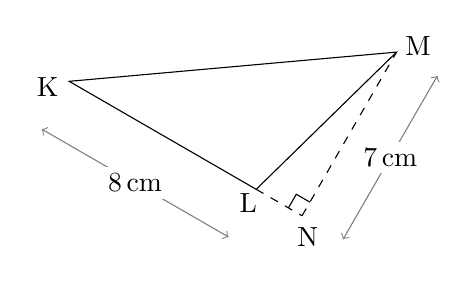
\begin{tikzpicture}[scale=1.0, baseline=(current bounding box.north)]
        \begin{scope}[rotate=-30]

        \coordinate (K) at (0,0);
        \coordinate (L) at (2.743,0);
        \coordinate (N) at ($(L)+(0.672,0)$);  % extend out
        \coordinate (M) at ($(N)+(0,2.4)$); % Perpendicular upwards

        \draw (K)--(L)--(M)--cycle;
        \draw[dashed] (L)--(N);
        \draw[dashed] (N)--(M);
        \pic [draw, -, angle radius=0.2cm] {right angle=M--N--L};

        % Vertex LABELS
        % Labels relative to shape geometry
        \node at ($(K)+(-0.2,-0.2)$) {K};
        \node at ($(L)+(0.0,-0.2)$) {L};
        \node at ($(N)+(0.2,-0.2)$) {N};
        \node at ($(M)+(0.2,0.2)$) {M};


        % dotted/dashed arrows shifted away from edges
        % Horizontal side (A-B), shifted down yshift=0mm,
        \draw[<->, gray]
            ($(K) + (0,-0.7cm)$) -- ($(L) + (0,-0.7cm)$)
            node[black, midway, fill=white, inner sep=2.5pt] {8\,cm};

        % Vertical side (D-C), shifted right xshift=0mm,
        \draw[<->, gray]
            ($(N)+(0.6,0)$) -- ($(N |- M)+(0.6,0)$)
            node[black, midway, fill=white, inner sep=2.5pt] {7\,cm};
    \end{scope}
\end{tikzpicture}
\end{minipage}%
\hfill
\begin{minipage}{.4\textwidth}
  \begin{align*}
    \text{Area} &= \frac{1}{2} \text{bh} \\
    \text{Area} &= \frac{1}{2} \times 8 \text{cm} \times 7 \text{cm}  \\
    \text{Area} &= \dotuline{~~~~~~~} \text{cm}^2
  \end{align*}
\end{minipage}

\par\vspace{1cm}\begin{minipage}{0.55\textwidth}
  \refstepcounter{minipagecount}
  \noindent{(\theminipagecount)}\quad
 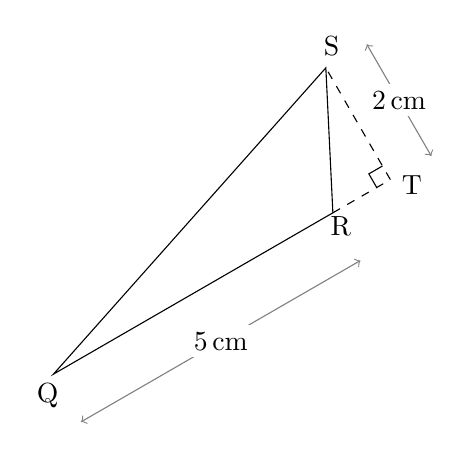
\begin{tikzpicture}[scale=1.0, baseline=(current bounding box.north)]
        \begin{scope}[rotate=30]

        \coordinate (Q) at (0,0);
        \coordinate (R) at (4.098,0);
        \coordinate (T) at ($(R)+(0.843,0)$);  % extend out
        \coordinate (S) at ($(T)+(0,1.639)$); % Perpendicular upwards

        \draw (Q)--(R)--(S)--cycle;
        \draw[dashed] (R)--(T);
        \draw[dashed] (T)--(S);
        \pic [draw, -, angle radius=0.2cm] {right angle=S--T--R};

        % Vertex LABELS
        % Labels relative to shape geometry
        \node at ($(Q)+(-0.2,-0.2)$) {Q};
        \node at ($(R)+(0.0,-0.2)$) {R};
        \node at ($(T)+(0.2,-0.2)$) {T};
        \node at ($(S)+(0.2,0.2)$) {S};


        % dotted/dashed arrows shifted away from edges
        % Horizontal side (A-B), shifted down yshift=0mm,
        \draw[<->, gray]
            ($(Q) + (0,-0.7cm)$) -- ($(R) + (0,-0.7cm)$)
            node[black, midway, fill=white, inner sep=2.5pt] {5\,cm};

        % Vertical side (D-C), shifted right xshift=0mm,
        \draw[<->, gray]
            ($(T)+(0.6,0)$) -- ($(T |- S)+(0.6,0)$)
            node[black, midway, fill=white, inner sep=2.5pt] {2\,cm};
    \end{scope}
\end{tikzpicture}
\end{minipage}%
\hfill
\begin{minipage}{.4\textwidth}
  \begin{align*}
    \text{Area} &= \frac{1}{2} \text{bh} \\
    \text{Area} &= \frac{1}{2} \times 5 \text{cm} \times 2 \text{cm}  \\
    \text{Area} &= \dotuline{~~~~~~~} \text{cm}^2
  \end{align*}
\end{minipage}

\par\vspace{1cm}\begin{minipage}{0.55\textwidth}
  \refstepcounter{minipagecount}
  \noindent{(\theminipagecount)}\quad
 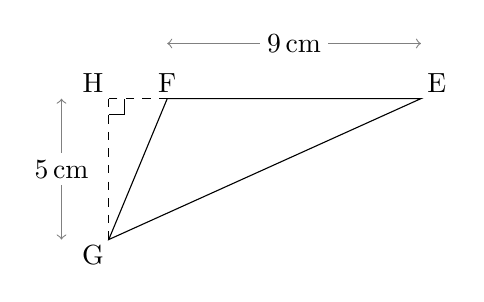
\begin{tikzpicture}[scale=1.0, baseline=(current bounding box.north)]
        \begin{scope}[rotate=180]

        \coordinate (E) at (0,0);
        \coordinate (F) at (3.222,0);
        \coordinate (H) at ($(F)+(0.743,0)$);  % extend out
        \coordinate (G) at ($(H)+(0,1.79)$); % Perpendicular upwards

        \draw (E)--(F)--(G)--cycle;
        \draw[dashed] (F)--(H);
        \draw[dashed] (H)--(G);
        \pic [draw, -, angle radius=0.2cm] {right angle=G--H--F};

        % Vertex LABELS
        % Labels relative to shape geometry
        \node at ($(E)+(-0.2,-0.2)$) {E};
        \node at ($(F)+(0.0,-0.2)$) {F};
        \node at ($(H)+(0.2,-0.2)$) {H};
        \node at ($(G)+(0.2,0.2)$) {G};


        % dotted/dashed arrows shifted away from edges
        % Horizontal side (A-B), shifted down yshift=0mm,
        \draw[<->, gray]
            ($(E) + (0,-0.7cm)$) -- ($(F) + (0,-0.7cm)$)
            node[black, midway, fill=white, inner sep=2.5pt] {9\,cm};

        % Vertical side (D-C), shifted right xshift=0mm,
        \draw[<->, gray]
            ($(H)+(0.6,0)$) -- ($(H |- G)+(0.6,0)$)
            node[black, midway, fill=white, inner sep=2.5pt] {5\,cm};
    \end{scope}
\end{tikzpicture}
\end{minipage}%
\hfill
\begin{minipage}{.4\textwidth}
  \begin{align*}
    \text{Area} &= \frac{1}{2} \text{bh} \\
    \text{Area} &= \frac{1}{2} \times 9 \text{cm} \times 5 \text{cm}  \\
    \text{Area} &= \dotuline{~~~~~~~} \text{cm}^2
  \end{align*}
\end{minipage}

\par\vspace{1cm}\begin{minipage}{0.55\textwidth}
  \refstepcounter{minipagecount}
  \noindent{(\theminipagecount)}\quad
 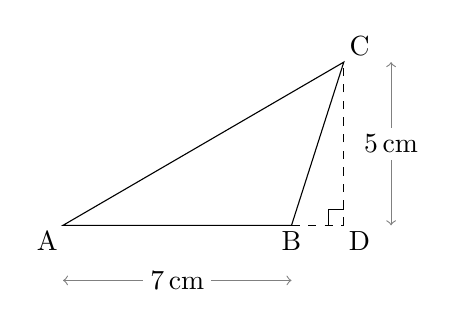
\begin{tikzpicture}[scale=1.0, baseline=(current bounding box.north)]
        \begin{scope}[rotate=0]

        \coordinate (A) at (0,0);
        \coordinate (B) at (2.902,0);
        \coordinate (D) at ($(B)+(0.664,0)$);  % extend out
        \coordinate (C) at ($(D)+(0,2.073)$); % Perpendicular upwards

        \draw (A)--(B)--(C)--cycle;
        \draw[dashed] (B)--(D);
        \draw[dashed] (D)--(C);
        \pic [draw, -, angle radius=0.2cm] {right angle=C--D--B};

        % Vertex LABELS
        % Labels relative to shape geometry
        \node at ($(A)+(-0.2,-0.2)$) {A};
        \node at ($(B)+(0.0,-0.2)$) {B};
        \node at ($(D)+(0.2,-0.2)$) {D};
        \node at ($(C)+(0.2,0.2)$) {C};


        % dotted/dashed arrows shifted away from edges
        % Horizontal side (A-B), shifted down yshift=0mm,
        \draw[<->, gray]
            ($(A) + (0,-0.7cm)$) -- ($(B) + (0,-0.7cm)$)
            node[black, midway, fill=white, inner sep=2.5pt] {7\,cm};

        % Vertical side (D-C), shifted right xshift=0mm,
        \draw[<->, gray]
            ($(D)+(0.6,0)$) -- ($(D |- C)+(0.6,0)$)
            node[black, midway, fill=white, inner sep=2.5pt] {5\,cm};
    \end{scope}
\end{tikzpicture}
\end{minipage}%
\hfill
\begin{minipage}{.4\textwidth}
  \begin{align*}
    \text{Area} &= \frac{1}{2} \text{bh} \\
    \text{Area} &= \frac{1}{2} \times 7 \text{cm} \times 5 \text{cm}  \\
    \text{Area} &= \dotuline{~~~~~~~} \text{cm}^2
  \end{align*}
\end{minipage}

\par\vspace{1cm}\begin{minipage}{0.55\textwidth}
  \refstepcounter{minipagecount}
  \noindent{(\theminipagecount)}\quad
 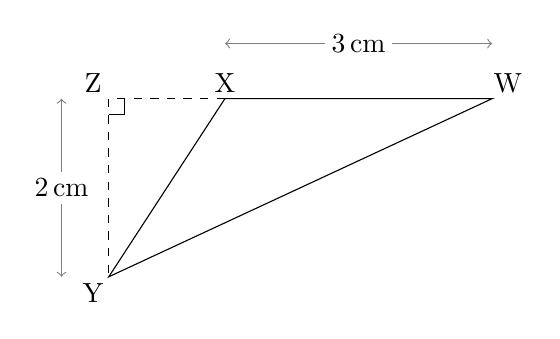
\begin{tikzpicture}[scale=1.0, baseline=(current bounding box.north)]
        \begin{scope}[rotate=180]

        \coordinate (W) at (0,0);
        \coordinate (X) at (3.394,0);
        \coordinate (Z) at ($(X)+(1.476,0)$);  % extend out
        \coordinate (Y) at ($(Z)+(0,2.263)$); % Perpendicular upwards

        \draw (W)--(X)--(Y)--cycle;
        \draw[dashed] (X)--(Z);
        \draw[dashed] (Z)--(Y);
        \pic [draw, -, angle radius=0.2cm] {right angle=Y--Z--X};

        % Vertex LABELS
        % Labels relative to shape geometry
        \node at ($(W)+(-0.2,-0.2)$) {W};
        \node at ($(X)+(0.0,-0.2)$) {X};
        \node at ($(Z)+(0.2,-0.2)$) {Z};
        \node at ($(Y)+(0.2,0.2)$) {Y};


        % dotted/dashed arrows shifted away from edges
        % Horizontal side (A-B), shifted down yshift=0mm,
        \draw[<->, gray]
            ($(W) + (0,-0.7cm)$) -- ($(X) + (0,-0.7cm)$)
            node[black, midway, fill=white, inner sep=2.5pt] {3\,cm};

        % Vertical side (D-C), shifted right xshift=0mm,
        \draw[<->, gray]
            ($(Z)+(0.6,0)$) -- ($(Z |- Y)+(0.6,0)$)
            node[black, midway, fill=white, inner sep=2.5pt] {2\,cm};
    \end{scope}
\end{tikzpicture}
\end{minipage}%
\hfill
\begin{minipage}{.4\textwidth}
  \begin{align*}
    \text{Area} &= \frac{1}{2} \text{bh} \\
    \text{Area} &= \frac{1}{2} \times 3 \text{cm} \times 2 \text{cm}  \\
    \text{Area} &= \dotuline{~~~~~~~} \text{cm}^2
  \end{align*}
\end{minipage}

\par\vspace{1cm}\begin{minipage}{0.55\textwidth}
  \refstepcounter{minipagecount}
  \noindent{(\theminipagecount)}\quad
 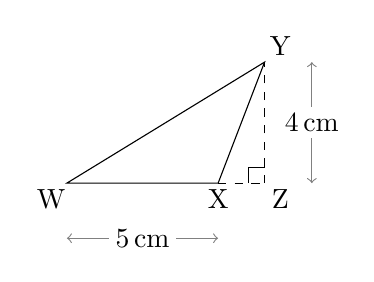
\begin{tikzpicture}[scale=1.0, baseline=(current bounding box.north)]
        \begin{scope}[rotate=0]

        \coordinate (W) at (0,0);
        \coordinate (X) at (1.921,0);
        \coordinate (Z) at ($(X)+(0.59,0)$);  % extend out
        \coordinate (Y) at ($(Z)+(0,1.537)$); % Perpendicular upwards

        \draw (W)--(X)--(Y)--cycle;
        \draw[dashed] (X)--(Z);
        \draw[dashed] (Z)--(Y);
        \pic [draw, -, angle radius=0.2cm] {right angle=Y--Z--X};

        % Vertex LABELS
        % Labels relative to shape geometry
        \node at ($(W)+(-0.2,-0.2)$) {W};
        \node at ($(X)+(0.0,-0.2)$) {X};
        \node at ($(Z)+(0.2,-0.2)$) {Z};
        \node at ($(Y)+(0.2,0.2)$) {Y};


        % dotted/dashed arrows shifted away from edges
        % Horizontal side (A-B), shifted down yshift=0mm,
        \draw[<->, gray]
            ($(W) + (0,-0.7cm)$) -- ($(X) + (0,-0.7cm)$)
            node[black, midway, fill=white, inner sep=2.5pt] {5\,cm};

        % Vertical side (D-C), shifted right xshift=0mm,
        \draw[<->, gray]
            ($(Z)+(0.6,0)$) -- ($(Z |- Y)+(0.6,0)$)
            node[black, midway, fill=white, inner sep=2.5pt] {4\,cm};
    \end{scope}
\end{tikzpicture}
\end{minipage}%
\hfill
\begin{minipage}{.4\textwidth}
  \begin{align*}
    \text{Area} &= \frac{1}{2} \text{bh} \\
    \text{Area} &= \frac{1}{2} \times 5 \text{cm} \times 4 \text{cm}  \\
    \text{Area} &= \dotuline{~~~~~~~} \text{cm}^2
  \end{align*}
\end{minipage}

\par\vspace{1cm}\begin{minipage}{0.55\textwidth}
  \refstepcounter{minipagecount}
  \noindent{(\theminipagecount)}\quad
 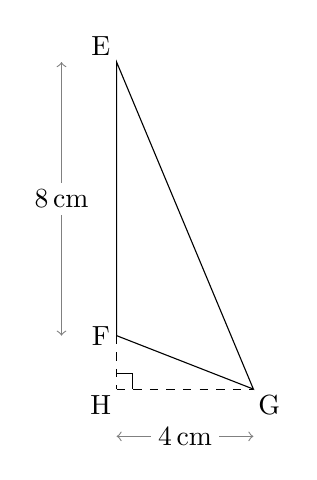
\begin{tikzpicture}[scale=1.0, baseline=(current bounding box.north)]
        \begin{scope}[rotate=270]

        \coordinate (E) at (0,0);
        \coordinate (F) at (3.474,0);
        \coordinate (H) at ($(F)+(0.679,0)$);  % extend out
        \coordinate (G) at ($(H)+(0,1.737)$); % Perpendicular upwards

        \draw (E)--(F)--(G)--cycle;
        \draw[dashed] (F)--(H);
        \draw[dashed] (H)--(G);
        \pic [draw, -, angle radius=0.2cm] {right angle=G--H--F};

        % Vertex LABELS
        % Labels relative to shape geometry
        \node at ($(E)+(-0.2,-0.2)$) {E};
        \node at ($(F)+(0.0,-0.2)$) {F};
        \node at ($(H)+(0.2,-0.2)$) {H};
        \node at ($(G)+(0.2,0.2)$) {G};


        % dotted/dashed arrows shifted away from edges
        % Horizontal side (A-B), shifted down yshift=0mm,
        \draw[<->, gray]
            ($(E) + (0,-0.7cm)$) -- ($(F) + (0,-0.7cm)$)
            node[black, midway, fill=white, inner sep=2.5pt] {8\,cm};

        % Vertical side (D-C), shifted right xshift=0mm,
        \draw[<->, gray]
            ($(H)+(0.6,0)$) -- ($(H |- G)+(0.6,0)$)
            node[black, midway, fill=white, inner sep=2.5pt] {4\,cm};
    \end{scope}
\end{tikzpicture}
\end{minipage}%
\hfill
\begin{minipage}{.4\textwidth}
  \begin{align*}
    \text{Area} &= \frac{1}{2} \text{bh} \\
    \text{Area} &= \frac{1}{2} \times 8 \text{cm} \times 4 \text{cm}  \\
    \text{Area} &= \dotuline{~~~~~~~} \text{cm}^2
  \end{align*}
\end{minipage}

\par\vspace{1cm}\begin{minipage}{0.55\textwidth}
  \refstepcounter{minipagecount}
  \noindent{(\theminipagecount)}\quad
 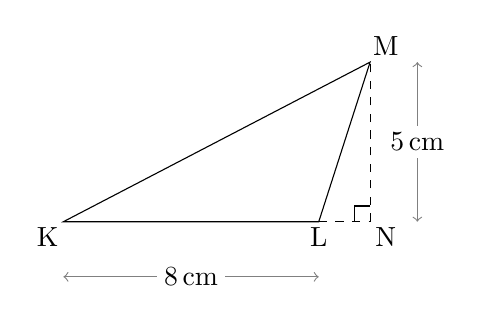
\begin{tikzpicture}[scale=1.0, baseline=(current bounding box.north)]
        \begin{scope}[rotate=0]

        \coordinate (K) at (0,0);
        \coordinate (L) at (3.243,0);
        \coordinate (N) at ($(L)+(0.652,0)$);  % extend out
        \coordinate (M) at ($(N)+(0,2.027)$); % Perpendicular upwards

        \draw (K)--(L)--(M)--cycle;
        \draw[dashed] (L)--(N);
        \draw[dashed] (N)--(M);
        \pic [draw, -, angle radius=0.2cm] {right angle=M--N--L};

        % Vertex LABELS
        % Labels relative to shape geometry
        \node at ($(K)+(-0.2,-0.2)$) {K};
        \node at ($(L)+(0.0,-0.2)$) {L};
        \node at ($(N)+(0.2,-0.2)$) {N};
        \node at ($(M)+(0.2,0.2)$) {M};


        % dotted/dashed arrows shifted away from edges
        % Horizontal side (A-B), shifted down yshift=0mm,
        \draw[<->, gray]
            ($(K) + (0,-0.7cm)$) -- ($(L) + (0,-0.7cm)$)
            node[black, midway, fill=white, inner sep=2.5pt] {8\,cm};

        % Vertical side (D-C), shifted right xshift=0mm,
        \draw[<->, gray]
            ($(N)+(0.6,0)$) -- ($(N |- M)+(0.6,0)$)
            node[black, midway, fill=white, inner sep=2.5pt] {5\,cm};
    \end{scope}
\end{tikzpicture}
\end{minipage}%
\hfill
\begin{minipage}{.4\textwidth}
  \begin{align*}
    \text{Area} &= \frac{1}{2} \text{bh} \\
    \text{Area} &= \frac{1}{2} \times 8 \text{cm} \times 5 \text{cm}  \\
    \text{Area} &= \dotuline{~~~~~~~} \text{cm}^2
  \end{align*}
\end{minipage}

\par\vspace{1cm}\begin{minipage}{0.55\textwidth}
  \refstepcounter{minipagecount}
  \noindent{(\theminipagecount)}\quad
 \begin{tikzpicture}[scale=1.0, baseline=(current bounding box.north)]
        \begin{scope}[rotate=270]

        \coordinate (Q) at (0,0);
        \coordinate (R) at (5.209,0);
        \coordinate (T) at ($(R)+(1.424,0)$);  % extend out
        \coordinate (S) at ($(T)+(0,2.315)$); % Perpendicular upwards

        \draw (Q)--(R)--(S)--cycle;
        \draw[dashed] (R)--(T);
        \draw[dashed] (T)--(S);
        \pic [draw, -, angle radius=0.2cm] {right angle=S--T--R};

        % Vertex LABELS
        % Labels relative to shape geometry
        \node at ($(Q)+(-0.2,-0.2)$) {Q};
        \node at ($(R)+(0.0,-0.2)$) {R};
        \node at ($(T)+(0.2,-0.2)$) {T};
        \node at ($(S)+(0.2,0.2)$) {S};


        % dotted/dashed arrows shifted away from edges
        % Horizontal side (A-B), shifted down yshift=0mm,
        \draw[<->, gray]
            ($(Q) + (0,-0.7cm)$) -- ($(R) + (0,-0.7cm)$)
            node[black, midway, fill=white, inner sep=2.5pt] {9\,cm};

        % Vertical side (D-C), shifted right xshift=0mm,
        \draw[<->, gray]
            ($(T)+(0.6,0)$) -- ($(T |- S)+(0.6,0)$)
            node[black, midway, fill=white, inner sep=2.5pt] {4\,cm};
    \end{scope}
\end{tikzpicture}
\end{minipage}%
\hfill
\begin{minipage}{.4\textwidth}
  \begin{align*}
    \text{Area} &= \frac{1}{2} \text{bh} \\
    \text{Area} &= \frac{1}{2} \times 9 \text{cm} \times 4 \text{cm}  \\
    \text{Area} &= \dotuline{~~~~~~~} \text{cm}^2
  \end{align*}
\end{minipage}

\par\vspace{1cm}\begin{minipage}{0.55\textwidth}
  \refstepcounter{minipagecount}
  \noindent{(\theminipagecount)}\quad
 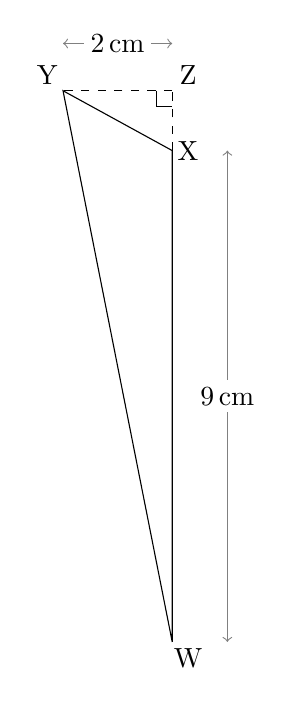
\begin{tikzpicture}[scale=1.0, baseline=(current bounding box.north)]
        \begin{scope}[rotate=90]

        \coordinate (W) at (0,0);
        \coordinate (X) at (6.24,0);
        \coordinate (Z) at ($(X)+(0.76,0)$);  % extend out
        \coordinate (Y) at ($(Z)+(0,1.387)$); % Perpendicular upwards

        \draw (W)--(X)--(Y)--cycle;
        \draw[dashed] (X)--(Z);
        \draw[dashed] (Z)--(Y);
        \pic [draw, -, angle radius=0.2cm] {right angle=Y--Z--X};

        % Vertex LABELS
        % Labels relative to shape geometry
        \node at ($(W)+(-0.2,-0.2)$) {W};
        \node at ($(X)+(0.0,-0.2)$) {X};
        \node at ($(Z)+(0.2,-0.2)$) {Z};
        \node at ($(Y)+(0.2,0.2)$) {Y};


        % dotted/dashed arrows shifted away from edges
        % Horizontal side (A-B), shifted down yshift=0mm,
        \draw[<->, gray]
            ($(W) + (0,-0.7cm)$) -- ($(X) + (0,-0.7cm)$)
            node[black, midway, fill=white, inner sep=2.5pt] {9\,cm};

        % Vertical side (D-C), shifted right xshift=0mm,
        \draw[<->, gray]
            ($(Z)+(0.6,0)$) -- ($(Z |- Y)+(0.6,0)$)
            node[black, midway, fill=white, inner sep=2.5pt] {2\,cm};
    \end{scope}
\end{tikzpicture}
\end{minipage}%
\hfill
\begin{minipage}{.4\textwidth}
  \begin{align*}
    \text{Area} &= \frac{1}{2} \text{bh} \\
    \text{Area} &= \frac{1}{2} \times 9 \text{cm} \times 2 \text{cm}  \\
    \text{Area} &= \dotuline{~~~~~~~} \text{cm}^2
  \end{align*}
\end{minipage}

\par\vspace{1cm}\begin{minipage}{0.55\textwidth}
  \refstepcounter{minipagecount}
  \noindent{(\theminipagecount)}\quad
 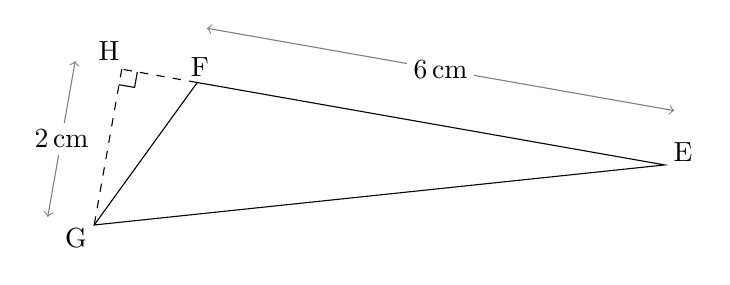
\begin{tikzpicture}[scale=1.0, baseline=(current bounding box.north)]
        \begin{scope}[rotate=170]

        \coordinate (E) at (0,0);
        \coordinate (F) at (6.027,0);
        \coordinate (H) at ($(F)+(0.973,0)$);  % extend out
        \coordinate (G) at ($(H)+(0,2.009)$); % Perpendicular upwards

        \draw (E)--(F)--(G)--cycle;
        \draw[dashed] (F)--(H);
        \draw[dashed] (H)--(G);
        \pic [draw, -, angle radius=0.2cm] {right angle=G--H--F};

        % Vertex LABELS
        % Labels relative to shape geometry
        \node at ($(E)+(-0.2,-0.2)$) {E};
        \node at ($(F)+(0.0,-0.2)$) {F};
        \node at ($(H)+(0.2,-0.2)$) {H};
        \node at ($(G)+(0.2,0.2)$) {G};


        % dotted/dashed arrows shifted away from edges
        % Horizontal side (A-B), shifted down yshift=0mm,
        \draw[<->, gray]
            ($(E) + (0,-0.7cm)$) -- ($(F) + (0,-0.7cm)$)
            node[black, midway, fill=white, inner sep=2.5pt] {6\,cm};

        % Vertical side (D-C), shifted right xshift=0mm,
        \draw[<->, gray]
            ($(H)+(0.6,0)$) -- ($(H |- G)+(0.6,0)$)
            node[black, midway, fill=white, inner sep=2.5pt] {2\,cm};
    \end{scope}
\end{tikzpicture}
\end{minipage}%
\hfill
\begin{minipage}{.4\textwidth}
  \begin{align*}
    \text{Area} &= \frac{1}{2} \text{bh} \\
    \text{Area} &= \frac{1}{2} \times 6 \text{cm} \times 2 \text{cm}  \\
    \text{Area} &= \dotuline{~~~~~~~} \text{cm}^2
  \end{align*}
\end{minipage}

\par\vspace{1cm}\begin{minipage}{0.55\textwidth}
  \refstepcounter{minipagecount}
  \noindent{(\theminipagecount)}\quad
 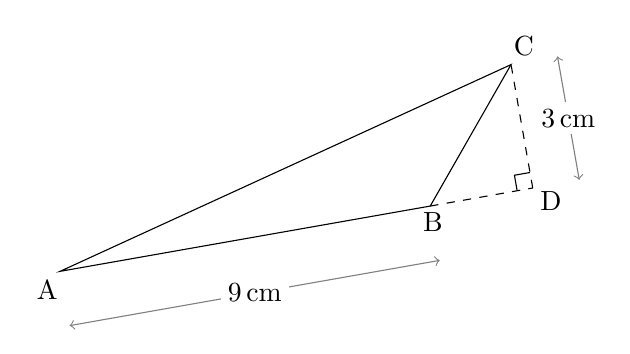
\begin{tikzpicture}[scale=1.0, baseline=(current bounding box.north)]
        \begin{scope}[rotate=10]

        \coordinate (A) at (0,0);
        \coordinate (B) at (4.773,0);
        \coordinate (D) at ($(B)+(1.321,0)$);  % extend out
        \coordinate (C) at ($(D)+(0,1.591)$); % Perpendicular upwards

        \draw (A)--(B)--(C)--cycle;
        \draw[dashed] (B)--(D);
        \draw[dashed] (D)--(C);
        \pic [draw, -, angle radius=0.2cm] {right angle=C--D--B};

        % Vertex LABELS
        % Labels relative to shape geometry
        \node at ($(A)+(-0.2,-0.2)$) {A};
        \node at ($(B)+(0.0,-0.2)$) {B};
        \node at ($(D)+(0.2,-0.2)$) {D};
        \node at ($(C)+(0.2,0.2)$) {C};


        % dotted/dashed arrows shifted away from edges
        % Horizontal side (A-B), shifted down yshift=0mm,
        \draw[<->, gray]
            ($(A) + (0,-0.7cm)$) -- ($(B) + (0,-0.7cm)$)
            node[black, midway, fill=white, inner sep=2.5pt] {9\,cm};

        % Vertical side (D-C), shifted right xshift=0mm,
        \draw[<->, gray]
            ($(D)+(0.6,0)$) -- ($(D |- C)+(0.6,0)$)
            node[black, midway, fill=white, inner sep=2.5pt] {3\,cm};
    \end{scope}
\end{tikzpicture}
\end{minipage}%
\hfill
\begin{minipage}{.4\textwidth}
  \begin{align*}
    \text{Area} &= \frac{1}{2} \text{bh} \\
    \text{Area} &= \frac{1}{2} \times 9 \text{cm} \times 3 \text{cm}  \\
    \text{Area} &= \dotuline{~~~~~~~} \text{cm}^2
  \end{align*}
\end{minipage}

\par\vspace{1cm}\begin{minipage}{0.55\textwidth}
  \refstepcounter{minipagecount}
  \noindent{(\theminipagecount)}\quad
 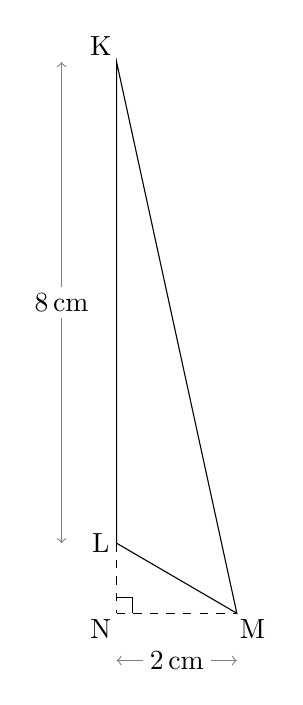
\begin{tikzpicture}[scale=1.0, baseline=(current bounding box.north)]
        \begin{scope}[rotate=270]

        \coordinate (K) at (0,0);
        \coordinate (L) at (6.11,0);
        \coordinate (N) at ($(L)+(0.89,0)$);  % extend out
        \coordinate (M) at ($(N)+(0,1.527)$); % Perpendicular upwards

        \draw (K)--(L)--(M)--cycle;
        \draw[dashed] (L)--(N);
        \draw[dashed] (N)--(M);
        \pic [draw, -, angle radius=0.2cm] {right angle=M--N--L};

        % Vertex LABELS
        % Labels relative to shape geometry
        \node at ($(K)+(-0.2,-0.2)$) {K};
        \node at ($(L)+(0.0,-0.2)$) {L};
        \node at ($(N)+(0.2,-0.2)$) {N};
        \node at ($(M)+(0.2,0.2)$) {M};


        % dotted/dashed arrows shifted away from edges
        % Horizontal side (A-B), shifted down yshift=0mm,
        \draw[<->, gray]
            ($(K) + (0,-0.7cm)$) -- ($(L) + (0,-0.7cm)$)
            node[black, midway, fill=white, inner sep=2.5pt] {8\,cm};

        % Vertical side (D-C), shifted right xshift=0mm,
        \draw[<->, gray]
            ($(N)+(0.6,0)$) -- ($(N |- M)+(0.6,0)$)
            node[black, midway, fill=white, inner sep=2.5pt] {2\,cm};
    \end{scope}
\end{tikzpicture}
\end{minipage}%
\hfill
\begin{minipage}{.4\textwidth}
  \begin{align*}
    \text{Area} &= \frac{1}{2} \text{bh} \\
    \text{Area} &= \frac{1}{2} \times 8 \text{cm} \times 2 \text{cm}  \\
    \text{Area} &= \dotuline{~~~~~~~} \text{cm}^2
  \end{align*}
\end{minipage}

\par\vspace{1cm}\begin{minipage}{0.55\textwidth}
  \refstepcounter{minipagecount}
  \noindent{(\theminipagecount)}\quad
 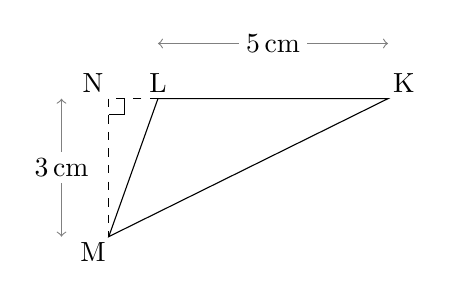
\begin{tikzpicture}[scale=1.0, baseline=(current bounding box.north)]
        \begin{scope}[rotate=180]

        \coordinate (K) at (0,0);
        \coordinate (L) at (2.922,0);
        \coordinate (N) at ($(L)+(0.625,0)$);  % extend out
        \coordinate (M) at ($(N)+(0,1.753)$); % Perpendicular upwards

        \draw (K)--(L)--(M)--cycle;
        \draw[dashed] (L)--(N);
        \draw[dashed] (N)--(M);
        \pic [draw, -, angle radius=0.2cm] {right angle=M--N--L};

        % Vertex LABELS
        % Labels relative to shape geometry
        \node at ($(K)+(-0.2,-0.2)$) {K};
        \node at ($(L)+(0.0,-0.2)$) {L};
        \node at ($(N)+(0.2,-0.2)$) {N};
        \node at ($(M)+(0.2,0.2)$) {M};


        % dotted/dashed arrows shifted away from edges
        % Horizontal side (A-B), shifted down yshift=0mm,
        \draw[<->, gray]
            ($(K) + (0,-0.7cm)$) -- ($(L) + (0,-0.7cm)$)
            node[black, midway, fill=white, inner sep=2.5pt] {5\,cm};

        % Vertical side (D-C), shifted right xshift=0mm,
        \draw[<->, gray]
            ($(N)+(0.6,0)$) -- ($(N |- M)+(0.6,0)$)
            node[black, midway, fill=white, inner sep=2.5pt] {3\,cm};
    \end{scope}
\end{tikzpicture}
\end{minipage}%
\hfill
\begin{minipage}{.4\textwidth}
  \begin{align*}
    \text{Area} &= \frac{1}{2} \text{bh} \\
    \text{Area} &= \frac{1}{2} \times 5 \text{cm} \times 3 \text{cm}  \\
    \text{Area} &= \dotuline{~~~~~~~} \text{cm}^2
  \end{align*}
\end{minipage}

\par\vspace{1cm}\begin{minipage}{0.55\textwidth}
  \refstepcounter{minipagecount}
  \noindent{(\theminipagecount)}\quad
 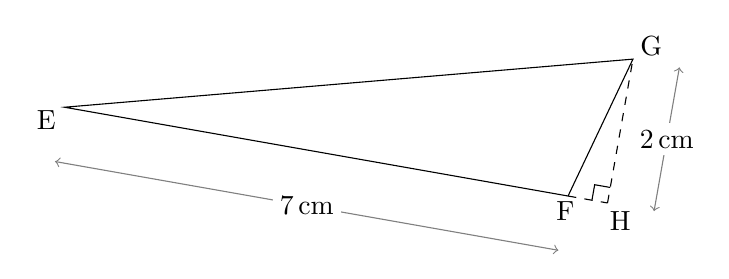
\begin{tikzpicture}[scale=1.0, baseline=(current bounding box.north)]
        \begin{scope}[rotate=-10]

        \coordinate (E) at (0,0);
        \coordinate (F) at (6.492,0);
        \coordinate (H) at ($(F)+(0.508,0)$);  % extend out
        \coordinate (G) at ($(H)+(0,1.855)$); % Perpendicular upwards

        \draw (E)--(F)--(G)--cycle;
        \draw[dashed] (F)--(H);
        \draw[dashed] (H)--(G);
        \pic [draw, -, angle radius=0.2cm] {right angle=G--H--F};

        % Vertex LABELS
        % Labels relative to shape geometry
        \node at ($(E)+(-0.2,-0.2)$) {E};
        \node at ($(F)+(0.0,-0.2)$) {F};
        \node at ($(H)+(0.2,-0.2)$) {H};
        \node at ($(G)+(0.2,0.2)$) {G};


        % dotted/dashed arrows shifted away from edges
        % Horizontal side (A-B), shifted down yshift=0mm,
        \draw[<->, gray]
            ($(E) + (0,-0.7cm)$) -- ($(F) + (0,-0.7cm)$)
            node[black, midway, fill=white, inner sep=2.5pt] {7\,cm};

        % Vertical side (D-C), shifted right xshift=0mm,
        \draw[<->, gray]
            ($(H)+(0.6,0)$) -- ($(H |- G)+(0.6,0)$)
            node[black, midway, fill=white, inner sep=2.5pt] {2\,cm};
    \end{scope}
\end{tikzpicture}
\end{minipage}%
\hfill
\begin{minipage}{.4\textwidth}
  \begin{align*}
    \text{Area} &= \frac{1}{2} \text{bh} \\
    \text{Area} &= \frac{1}{2} \times 7 \text{cm} \times 2 \text{cm}  \\
    \text{Area} &= \dotuline{~~~~~~~} \text{cm}^2
  \end{align*}
\end{minipage}

\par\vspace{1cm}

\end{document}
